\chapter{Tutorial on Factor graph state estimation}
\minitoc

Let us explicit the terms prevent in this chapter's title. 

The \textit{state} of the robot is a set of variables of particular interest to the roboticist, be it for control, parameter identification, etc.
Those quantities may not directly measurable, due to their physical nature (an angular momentum sensor would be hard to imagine) or because sensor data
is too noisy, biased, or impractical to obtain (eg. GPS for localization is very bad close to flat surfaces because of beam reflections). 
Those latent variables can however be estimated by fusing multiple sensors data using a state estimator (aka. observer in automation). In the context of 
a probabilistic estimator, these are random variables. Most state estimators work with variables which sample state is continuous. The goal is then 
to find the probability density of those states.

Taking the Bayesian perspective, the most general problem is to find a distribution over a collection of random variables $\mathcal{X}$ given a set 
of measurements $\mathcal{Z}$, $p(\mathcal{X} | \mathcal{Z})$ which is known as the \textit{posterior}. 
The Bayes law represents this exact inference:
%
\begin{equation}
    p(\mathcal{X} | \mathcal{Z}) = \frac{p(\mathcal{Z} | \mathcal{X}) p(\mathcal{X})}{p(\mathcal{Z})} 
\end{equation}
%
$p(\mathcal{Z} | \mathcal{X})$ is the measurement model that can be obtained through modeling, also called the \textit{likelihood} of the observation. 
$p(\mathcal{X})$ is a \textit{prior} that we have on the state variable distribution. This may include for instance knowledge about the initial state of the robot or
an approximate value of parameters that we seek to estimate.
The \textit{partition constant} $p(\mathcal{Z})$ can be thought of as a global normalization constant (\cite{koller2009probabilistic}, chapter 20 ) in case 
the $\mathcal{Z}$ random variable is observed, which is our case. In general, this term is computationally intractable to compute. Exact inference is 
therefore rarely undertaken, instead relying on approximate inference methods such as variational inference (\cite{koller2009probabilistic}, chapter 11) 
or sampling (\cite{koller2009probabilistic}, chapter 12). In the context of robotics, sampling has been leveraged in the popular particle filter which for 
tasks such as localization \cite{dellaert1999monte} and SLAM \cite{montemerlo2002fastslam}. Application of variational inference is scarcer, with the notable 
exceptions of works from Barfoot \cite{barfoot2020exactly, wong2020variational} which derives a graph optimization estimation based on variational inference
and Lambert \cite{lambert2022recursive} which proposes a recursive variational Gaussian filter.

However full Bayesian inference is not always required in robotics contexts, as we are often mainly interested in the most probable state.

\section{Maximum A Posteriori estimation}

A more popular approach to the estimation problem is to solve the \textit{Maximum A Posteriori} (MAP) problem. Instead of finding the full posterior, we are most often only 
interested in finding the most likely state which corresponds to solving the optimization problem:
%
\begin{equation}
    \label{eq:MAP_pbe}
    \mathcal{X}^* \triangleq \argmax_{\mathcal{X}} p(\mathcal{X} | \mathcal{Z}) = \argmax_{\mathcal{X}} p(\mathcal{Z} | \mathcal{X}) p(\mathcal{X}),
\end{equation}
%
$p(\mathcal{Z})$, being constant with respect to $\mathcal{X}$.

Additional assumptions have to be made in order to obtain a numerical implementation of this problem.
First, the measurements $\mathcal{Z} = \{\bfz_0, \bfz_1, ..., \bfz_N\} $, which are a set of individual sensor observations, that are supposed to be conditionally 
independent of each other, so that the likelihood function can be factorized. 
%
\begin{equation}
    p(\mathcal{Z} | \mathcal{X}) p(\mathcal{X}) = \prod^{N} p(\bfz_i | \mathcal{X}_{S_i}) p(\mathcal{X}_0)
\end{equation}
%
Each factor represents the measurement model associated to the 
observation $\bfz_i$ and depending only on a subset $S_i$ of the state variables $\mathcal{X}_{S_i}$. 
$\mathcal{X}_0$ denotes the subset of random variables on which we have nonuniform prior.
Secondly, these measurement models are assumed to multivariate Gaussian distributions:
%
\begin{equation}
    p(\bfz_i | \mathcal{X}_{S_i}) = \frac{1}{\sqrt{2\pi\Sigma_i}} ~ \exp(- \frac{1}{2} (||\bfr_i(X_{S_i})||_{\Sigma_i}) \triangleq K_i~\phi_i(\mathcal{X}_{S_i})
\end{equation}
%
where the \textit{residuals} $\bfr_i$ are (potentially) nonlinear functions of the state variables, $K_i$ are constants, $\Sigma_i$ is the covariance of the observation noise,
$\phi_i(\mathcal{X}_{S_i})$ is the un-normalized measurement likelihoods called \textit{factors},
and 
%
\begin{equation*}
    ||\bfr_i(X_{S_i})||_{\Sigma_i} = \bfr_i(X_{S_i}) \Sigma_i^{-1} \bfr_i(X_{S_i})    
\end{equation*}
%
is known as the Mahalanobis distance. 
Residuals $\bfr_i(X_{S_i})$ can generally be formulated as a difference between a \textit{expectation function} $\bfh$ and the actual measurements
%
\begin{equation}
    \bfr_i(X_{S_i}) = \bfh(\mathcal{X}_{S_i}) \ominus \bfz_i,
\end{equation}
%
where $\ominus$ is a generalized difference operator,
although some exceptions may exist (see for instance \eqRef{eq:preint_residual} in \secRef{sec:preint_residual}).
%
Thus, the posterior probability is proportional to a product of individual factors:
%
\begin{equation}
    p(\mathcal{X} | \mathcal{Z}) \propto \phi_i(X_{S_i}) \phi_0(\mathcal{X}_{0})
    \label{eq:likelihood_factorization}
\end{equation}
%
Recognizing than maximizing the likelihood in \eqRef{eq:MAP_pbe} is equivalent to minimizing the negative log-likelihood.
%
\begin{align}
    \mathcal{X}^* 
    &= \argmin_{\mathcal{X}} - \log p(\mathcal{Z} | \mathcal{X}) ~&\mbox{\small MAP problem definition}\\
    &= \argmin_{\mathcal{X}} - \log p(\mathcal{Z} | \mathcal{X}) p(\mathcal{X}) ~&\mbox{\small Unaffected Partition constant}\\
    &= \argmin_{\mathcal{X}} - \log \prod^{N} p(\bfz_i | \mathcal{X}_{S_i}) p(\mathcal{X}_0) ~&\mbox{\small Conditional independences}\\
    &= \argmin_{\mathcal{X}} - \log \prod^{N} \phi_i(X_{S_i}) \phi_0(\mathcal{X}_{0}) ~&\mbox{\small Factorized likelihood}\\
    &= \argmin_{\mathcal{X}} \sum^{N} ||\bfr_i(\mathcal{X}_{S_i})||_{\Sigma_i}^2 + ||\bfr_0(\mathcal{X}_{0})||_{\Sigma_0}^2 ~&\mbox{\small Gaussian measurement models}\\
\end{align}

Thus, solving the MAP problem with the aforementioned hypothesis boils down to solving a nonlinear least-squares (NLLS) problem. 
A vast part of the literature on MAP estimation has been dedicated to the implementation of efficient solvers. Most of them are 
gradient-based algorithm, typically some variation of the Gauss-Newton algorithm, such as the Levenberg-Marquardt algorithm \cite{boyd2004convex}.


\section{Factor Graphs: a visual language for robotics estimation}
A crucial aspect of solving the MAP problem is the factorizibility of the likelihood function. This represents the fact that the problem
exhibits a particular structure that has important computational implications. Let's consider the toy example represented in \figRef{fig:toy_problem}. 
We wish to estimate the trajectory of a differential robot, that is its states at chosen timestamps called \textit{\keyframes}, and \textit{landmarks} which are elements of the 
environment that are easily detectable. We suppose that this robot is equipped with an odometer, which measurements integrated over time provide relative 
transformations between \keyframes, and an exteroceptive sensor, which provides relative measurements between \keyframes landmarks.

\begin{figure}[h]
    \centering
    \begin{subfigure}{.49\linewidth}
        \centering
        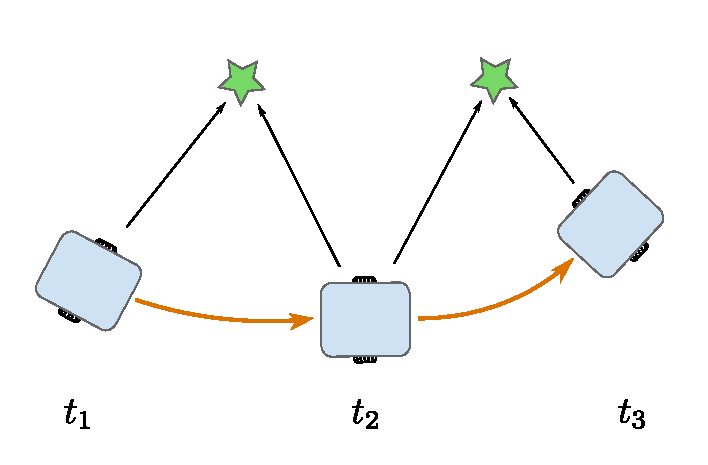
\includegraphics[width=\textwidth]{figures/toy_example.pdf}
        \caption{\label{fig:toy_problem}}
    \end{subfigure}%
    \hfill
    \begin{subfigure}{.49\linewidth}
        \centering
        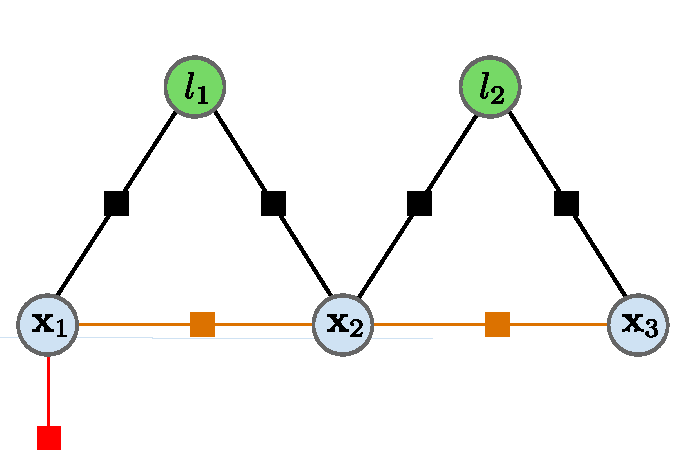
\includegraphics[width=\textwidth]{figures/toy_factor.pdf}
        \caption{\label{fig:toy_factor}}
    \end{subfigure}%
    \caption{(\subref{fig:toy_problem}): toy estimation problem, a differential drive robot equipped with an odometer moves in 
    an scene with landmarks represented by stars. \subref{fig:toy_factor}): Factor Graph representation the problem, the estimated variables are represented by circles 
    (blue for robot \keyframe, green for landmarks) and factors by squares (orange for odometry, black for exteroceptive sensor).}
\end{figure}

In this case, the state variables are $\mathcal{X} = \{ \bfx_1, \bfx_2, \bfx_3, l_1, l_2\}$ %and measurements $\mathcal{Z} = \{ z_{o,1}, z_{o,2}, z_{e,1}, z_{e,2}\}$
We also apply a prior on the pose of the first \keyframe of the trajectory, which can be understood as fixing the frame origin of the reference 
frame in which the estimation is done.

The factorization of the likelihood of \eqRef{eq:likelihood_factorization} in this example writes:
%
\begin{align}
    p(\mathcal{X} | \mathcal{Z}) \propto 
    &{\color{Red} \phi_0({\color{Blue} \bfx_{0}})} \\ 
    &{\color{Orange} \phi_1({\color{Blue} \bfx_1}, {\color{Blue} \bfx_2}) \phi_2({\color{Blue} \bfx_2}, {\color{Blue} \bfx_3})} \\ 
    &{\color{Black} \phi_3({\color{Blue} \bfx_1}, {\color{Green} l_1}) \phi_4({\color{Blue} \bfx_2}, {\color{Green} l_1}, {\color{Green} l_2}) \phi_5({\color{Blue} \bfx_3}, {\color{Green} l_2})} \\ 
\end{align}
%
This factorization can be represented as a \textit{Factor Graph} as seen in \ref{fig:toy_factor}. 
Factor Graphs are popular graphical models \cite{koller2009probabilistic} that can describe a vast family of statistical models \cite{loeliger2004introduction}.
A Factor Graph in the most general sense is a bipartite graph that represents the factorization of a function of several variables. 
We adopt the visual notation commonly found in robotics: round nodes for variables, square nods for factors, edges represent the dependency 
of each factor on a subset of variables. Over the last two decades, they have grown in popularity among roboticists as a visual language to describe 
estimation problems \cite{dellaert2017factor} and planning problem \cite{dong2016motion}. Dellaert and Kaess \cite{dellaert2006square} were the first to
recognize the link between NLLS problems and Factor graph.

Many specialized solvers \cite{grisetti2011g2o, dellaert2012factor, ila2017slam++} have been implemented that exploit the sparse structure of these 
problems. A discussion of the particularities of Factor Graph based NNLS solvers can be found in [CITE sola course] \cite{dellaert2017factor}.


% \section{Lie groups primers}
% - very short introduction of the exponential map
